\documentclass[a4paper,11pt]{article}
\usepackage[utf8]{inputenc}
\usepackage[T1]{fontenc}
\usepackage[a4paper,top=1in, bottom=1in, left=1in, right=1in]{geometry}
\usepackage[french,magyar]{babel}
\def\magyarOptions{defaults=prettiest}

\usepackage[none]{hyphenat}
\usepackage{amsfonts,amsmath,amssymb}
\usepackage{fancyhdr}
\usepackage[none]{hyphenat}

\usepackage[dvipsnames]{xcolor}
\usepackage[nottoc,notlot,notlof]{tocbibind}
\usepackage{graphicx}
\usepackage{caption}
\usepackage{subfig}
\usepackage{enumitem}
\usepackage{booktabs}
\usepackage[export]{adjustbox}
\usepackage{enumitem}
\setlist[1]{itemsep=-5pt}
\pagestyle{fancy}
\fancyhead{}
%\fancyfoot{}
\renewcommand{\headrulewidth}{0pt}

\usepackage{hyperref}

\usepackage{listings}
 
\urlstyle{same}

%\renewcommand{\baselinestretch}{1.5}

\begin{document}
%\emergencystretch 3em
\sloppy

\begin{titlepage}
\begin{center}
%\vspace{1cm}
\begin{figure}[t!]
	\begin{center}
	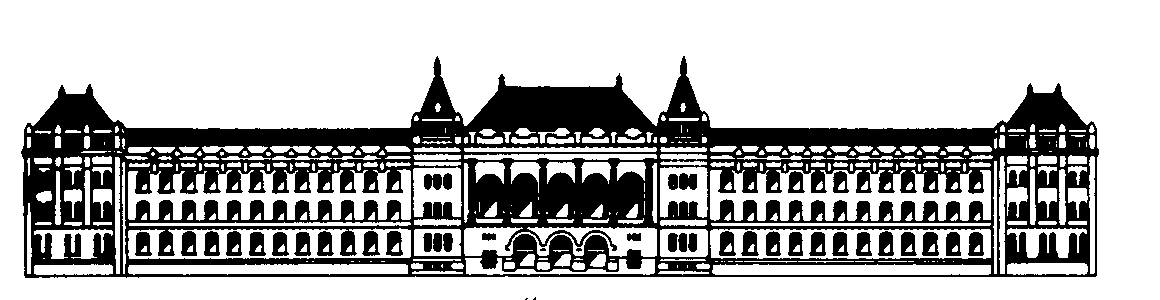
\includegraphics[scale=0.2]{bme.png}
	\label{a:bme}
	\end{center}
\end{figure}
\textbf{{Budapesti Műszaki és Gazdaságtudományi Egyetem}}\\
Villamosmérnöki és Informatikai Kar\\
Méréstechnika és Információs Rendszerek Tanszék\\
\vfill
\huge\textbf{{Logikai tervezés}}\\[3mm]
\Large{Házi feladat}\\[3mm]
\Large\textbf{{Programozható jelgenerátor}}\\
\vfill
\Large{Kardos Bálint, ZI84PX}\\
\Large{Murányi Péter, A74MW9}\\
\Large{Konzulens: Dr. Fehér Béla}\\
\vfill
\today \\

\end{center}
\end{titlepage}

\tableofcontents
\thispagestyle{empty}
\clearpage

\setcounter{page}{1}
\setcounter{tocdepth}{4}
\setcounter{secnumdepth}{4}
\setlength{\parindent}{2em}
%\setlength{\parskip}{1em}
\section{Feladat}

\section{Tervezés}

\section{Megvalósítás}
\subsection{DDS}

\subsection{Dithering}

\subsection{Toplevel}

\section{Forráskód}

\subsection{DDS}

\lstinputlisting[
language=Verilog,
inputencoding=latin1,
basicstyle=\fontsize{7}{13}\selectfont\ttfamily,
keywordstyle=\color{blue}\ttfamily,
commentstyle=\color{OliveGreen}\ttfamily,
backgroundcolor = \color{lightgray}
]{../DDS/DDS.srcs/sources_1/new/DDS_top.v}

\subsection{DDS toplevel}

\lstinputlisting[
language=Verilog,
inputencoding=latin1,
basicstyle=\fontsize{7}{13}\selectfont\ttfamily,
keywordstyle=\color{blue}\ttfamily,
commentstyle=\color{OliveGreen}\ttfamily,
backgroundcolor = \color{lightgray}
]{../DDS/DDS.srcs/sources_1/new/DDS_tl.v}


\pagebreak
\begin{thebibliography}{}

\bibitem{name1}

\textit{}
\url{  }
\today

\bibitem{name2}

\textit{}\\
\url{}
\today

\bibitem{name3}

\textit{}\\
\url{}
\today

\bibitem{name4}

\textit{}\\
\url{}
\today

\bibitem{name5}

\textit{}\\


\bibitem{name6}

\textit{}\\
\url{}
\today


\end{thebibliography}
\end{document}
